Approaches to differential abundance analysis have been controversial across the microbiome sciences.
The current gold standard requires laborious measurements of total biomass to accurately determine shifts
in microbial abundance among samples. Here, we highlight the pitfalls of comparing relative abundance across
samples and identify two solutions that reveal microbial changes without the need to estimate total biomass.
In an oral time series experiment, these methods alleviate false positives and produce consistent results
on both raw and cell count normalized data. Further, these methods identify differentially abundant
microbes previously undetectable with standard methods in two independent published atopic dermatitis
datasets. These methods therefore allow re-assessment of published relative abundance data to reveal
previously undetectable microbiome changes without the need for new molecular assays.
\section*{Introduction}
Next-generation microbiome sequencing provides data in the form of relative abundances,
independent of the total biomass of the original sample. Numerous analytical approaches
including rarefaction \cite{Weiss2015-gn}, median \cite{Love2014-sn}, and quantile normalization
\cite{Paulson2013-mm} have been proposed to make biological samples more comparable to each other.
However, these analytical solutions do not control for false discovery rates \cite{Russel2018-na},
\cite{Hawinkel2017-ax} and could even be a source of reproducibility issues observed in microbiome
studies \cite{Gloor2015-zq}. Here, we overcome these mathematical challenges in analyzing
compositional data in the context of microbiome sequencing data by presenting and utilizing
the notion of “reference frames” for inferring changes in abundance. We confirm our ability
to make the same inferences as one makes with absolute abundances by quantifying microbial load
in unstimulated saliva before and after brushing teeth, and analyzing 16S \gls{rrna} gene amplicon sequencing
data.  Finally, we analyze one published and one new skin metagenomic dataset and show that by analyzing
the ratios of taxa, or using a novel method of ranking taxa by their differential abundance as ratios of
proportions, we can find stable reference frames of compositional change and overcome the challenges
inherent in comparing relative abundances.\\[5 mm]
%
To illustrate pitfalls of comparing relative abundance data, consider the following toy example
in Figure 1. Here we have two samples collected  before and after a given treatment.  In the
scenario in Figure 1a, there are only two different taxa, colored orange and blue, that are in
equal proportions. The true sample is everything inside the large oval, but by sequencing we are
only observing a fraction of this sample, represented here by the taxa in the concentric dashed
oval labelled ‘observed’.  In the after treatment, we show two possible scenarios. Both observe
the same 2:1 ratio of orange to blue, and it is tempting to conclude from the relative abundances
that orange increased and blue decreased.  However, the true samples could differ dramatically
in their total microbial load. In the bottom scenario in Figure 1a, both orange and blue taxa
increase compared to the before sample, but the orange taxa increase more. Alternatively, in the
top scenario the number of orange taxa remains constant, and the number of blue taxa decrease.
Because we only observe an equal number of sequences, however, we cannot differentiate between
these two biologically important outcomes. In fact, there could be an infinite number of outcomes
that provide the same 2:1 ratio of orange to blue. This greatly complicates the generation of a
meaningful null hypothesis, and can cause misleading p-values if this phenomenon is not taken
into consideration.\\[5 mm]
\begin{figure}
  %%%\includegraphics{something} % this command will be ignored
  \centering
  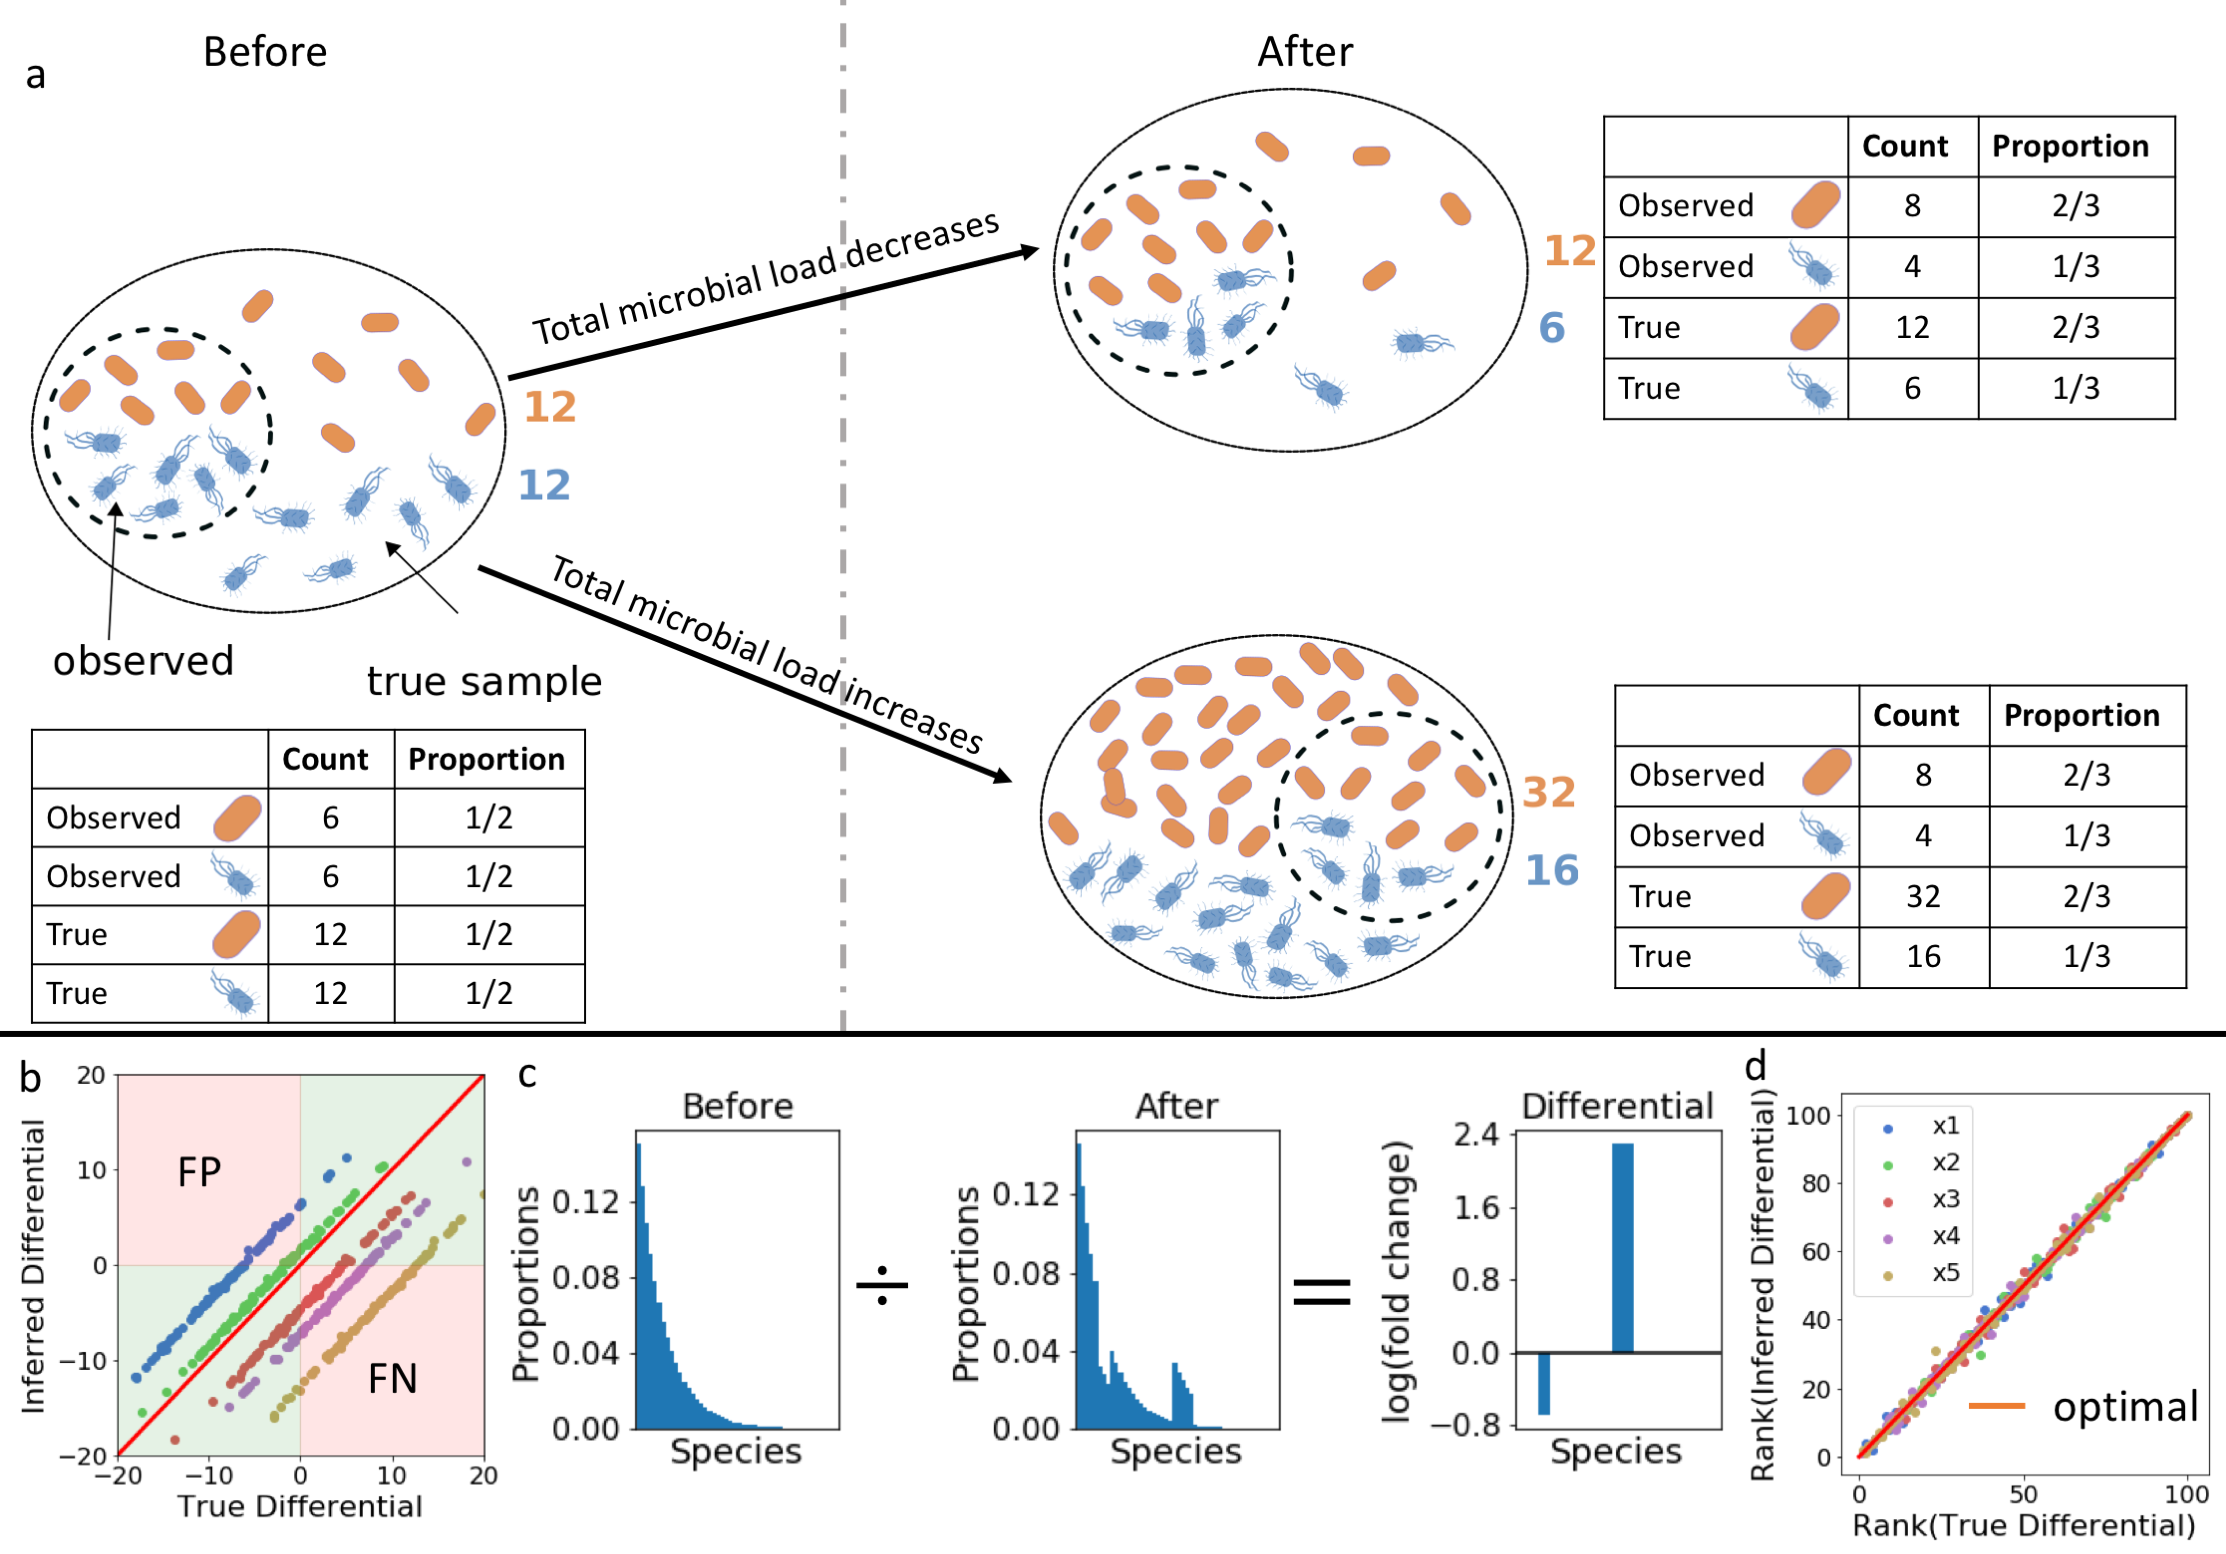
\includegraphics[width=1\textwidth]{ch4/Figure1.png}
  \caption[Illustration of total population size bias and the concept of differentials.]{
    Illustration demonstrating statistical limitations inherent to compositional datasets. (a) On the left,
    we have a scenario before a hypothetical treatment. On the right, we have a scenario after a hypothetical treatment.
    Two different scenarios can yield the exact same proportions in the after treatment. (b) Simulated datasets
    plotting the true differential from absolute data on the x-axis, versus the inferred differential from relative
    data on the y-axis. Each dot represents a taxa in the dataset, and the colors represent datasets with various
    ratios of total microbial load between before and after samples. The red line represents the optimal scenario
    where the samples have equal microbial load. This illustrates the prevalence of either false positives (\gls{fp}) or
    false negatives (\gls{fn}) when performing differential abundance analysis on samples with unequal total microbial load.
    The presence of either \gls{fp}s or \gls{fn}s is dictated by a nonlinear function of the true differential (see online methods).
    (c) An illustration of differential proportions of bacterial species before and after treatment. (d) Same data as
    (b) but plotting the rank of the differentials, demonstrating that ranks are equivalent independent of differences
    in microbial load.}
\end{figure}
%
%
Microbiome measurements from next-generation sequencing are inherently compositional. Samples are
typically collected from a much larger environment (e.g. fecal material from the gut, or water
sample from the ocean).  From these samples, a subset is separated for DNA extraction (e.g. swabbing
a fecal sample, or aliquoting a water sample). A subset of this DNA is then used as input for the PCR
reaction, and a subset of amplicon is pooled into a library, and a subset of the library is sequenced.
By the time that quality-filtered sequencing data is obtained, this data reflects only a small subset
of the true environment, and is not an accurate reflection of microbial load in the original sample
\cite{Vandeputte2017-jl}. Without knowledge of the total microbial load in the environment, we cannot
differentiate between the infinite number of possible scenarios governing which microbes increase and
decrease in abundance. This phenomenon has been shown to lead to close to 100\% false positive rates
in conventional statistical tools \cite{Mandal2015-xw,Morton2017-dz}.  \\[5 mm]
%
In order to properly infer true differences between individual microbes, one must measure the size of
the total population. This means that computing the change between samples using relative abundances
will introduce bias resulting from the lack of information concerning the total microbial load (online
methods Equation 2). Simulated data in Figure 1c shows how different biases (i.e. ratios between total
microbial loads) can cause either false positives or false negatives. \\[5 mm]
%
Multiple approaches at each level of sample processing have been proposed to quantify total microbial
load from environmental samples. At the sequencing level, adding a known amount of reference DNA not
expected to be present in the samples of interest has been used to extrapolate the amount of starting
material \cite{Smets2015-od, Tkacz2018-fp}.  Normalization by this method is complicated due to
calibration challenges of choosing the proper amount of internal standard \cite{Tkacz2018-fp,Smets2015-od}.
At the extraction level, quantitative PCR (\gls{qpcr}) of genomic DNA with ‘universal’ primers against the 16S
\gls{rrna} gene can be used to estimate total microbial load \cite{Nadkarni2002-og}. However, it is impossible
to escape primer bias because no perfect primer pair can equally amplify all \gls{rrna} genes across species.
Furthermore, both spike-in and \gls{qpcr} include the issue of various subsetting as discussed above. Finally,
quantifying microbial load with flow cytometry allows for evaluation of primary sample, and is agnostic
to nucleotide sequence. A recent study has shown that adding quantitative information from flow cytometry
to microbiome analyses can dramatically improve interpretation of 16S amplicon sequencing data
\cite{Vandeputte2017-jl}. However, this technique requires expensive equipment and experienced users,
and tends to be low throughput. \\[5 mm]
%
The absolute abundance of a community, however, is only one dimension of measurement among the hundreds
to thousands of dimensions measured in microbial relative abundances; if you know the abundance of a
single species, and the relative abundance of all species, you can compute the absolute abundance of
all species. As such, a lot of information rests in relative abundances and important insights can be
gleaned without costly absolute abundances. We show that through existing methods and a novel,
conceptually integrative method, one can make stable inferences of abundance changes without requiring
a costly and throughput-limiting single dimension measurement. We verify with mathematical proof and
empirical data that our inferences are equivalent to those obtained from data containing absolute abundances.\\[5 mm]
%
Analyzing compositional data requires choosing reference frames for inferring changes in abundance.
By “reference frames” , we draw on the concept from physics by which one measures velocity “relative to”
another moving object. The concepts are related, and provide a useful means of understanding how to make
stable inferences with compositional data. As microbial populations change, we can contain our inferences
to how microbial populations change relative to reference frames given by other microbial populations.\\[5 mm]
%
Compositional data are commonly analyzed using log-ratios, and the choice of numerator and denominator
in a log-ratio determines our reference frame for inferring changes. The “centered log-ratio” uses the
mean of all sequences as a reference frame, measuring changes of one species' abundance relative to the
mean of all species, analogous to astrophysicists measuring the movement of Earth relative to the center
of mass in the Milky Way. Log-odds analyses use “all other sequences” as a reference frame, measuring the
change of one species relative to the rest. Several recently developed tools for analyzing sequence count
data differ in the reference frames used for making inferences. Ph\gls{ilr} \cite{Silverman2016-he} uses sister
clades as reference frames for one-another. Phylofactorization\cite{Washburne2017-up} iteratively
partitions reference frames of species separated by edges in the phylogeny. Morton et al.
\cite{Morton2017-dz} found reference frames through hierarchical clustering.\\[5 mm]
%
Here, we empirically validate the stability of compositional tools for sequence count data analysis and
propose a rank-based method for illustrating the distribution of possible reference frames and discovering
useful pairwise references for making reliable inferences of abundance change in compositional sequence-count
data. By ranking the log-ratio abundance changes (what we refer to as the “differentials”), one obtains an
accurate image of compositional change in a dataset and one can visualize candidate reference frames for
inferring changes (Figure 1c). As shown in Figure 1d, ranking the differential is independent of the
changes in the absolute microbial load, yielding an identical ranking of microbial differences between the
relative and absolute abundances.\\[5 mm]
%
Differentials can be estimated directly from using explicit count-based regression models. For example,
multiple works \cite{Silverman2018-ql,Aijo2018-jp, Grantham2017-gv,Xia2013-nd} have shown that multinomial
generalized linear models can infer differentials without adding pseudocounts to handle sampling zeros.
When estimating differentials, one can't determine whether a particular species went up or down in absolute
abundance, but only whether one species' change is higher or lower than others. These differentials can be
interpreted as feature importances or rankings commonly employed by machine learning methods.\\[5 mm]
\section{Results}
\subsection{Absolute quantification of unstimulated saliva microbes}
%
We demonstrate the utility of employing such tools in a 16S \gls{rrna} gene amplicon dataset of saliva samples
under a familiar scenario (tooth brushing) with matching quantitative flow cytometry data for validation.
Unstimulated saliva samples were collected from 8 individuals before and after brushing their teeth
(morning and night, n=32), and processed in parallel for microbial load quantification with flow cytometry
and 16S \gls{rrna} gene amplicon sequencing. Importantly, participants were asked to provide unstimulated saliva
for exactly 5 minutes, so in addition to estimating microbial concentration, we could obtain a proxy for
total microbial load in 5 minutes by taking into account salivary flow rate. As expected, total microbial
load significantly decreased after brushing teeth (Fig. 2a). By using analytical tools appropriate to
compositional datasets, we get the same results for differential abundance whether or not we normalize
our sequencing data to account for the change in microbial load. \\[5 mm]
\begin{figure}
  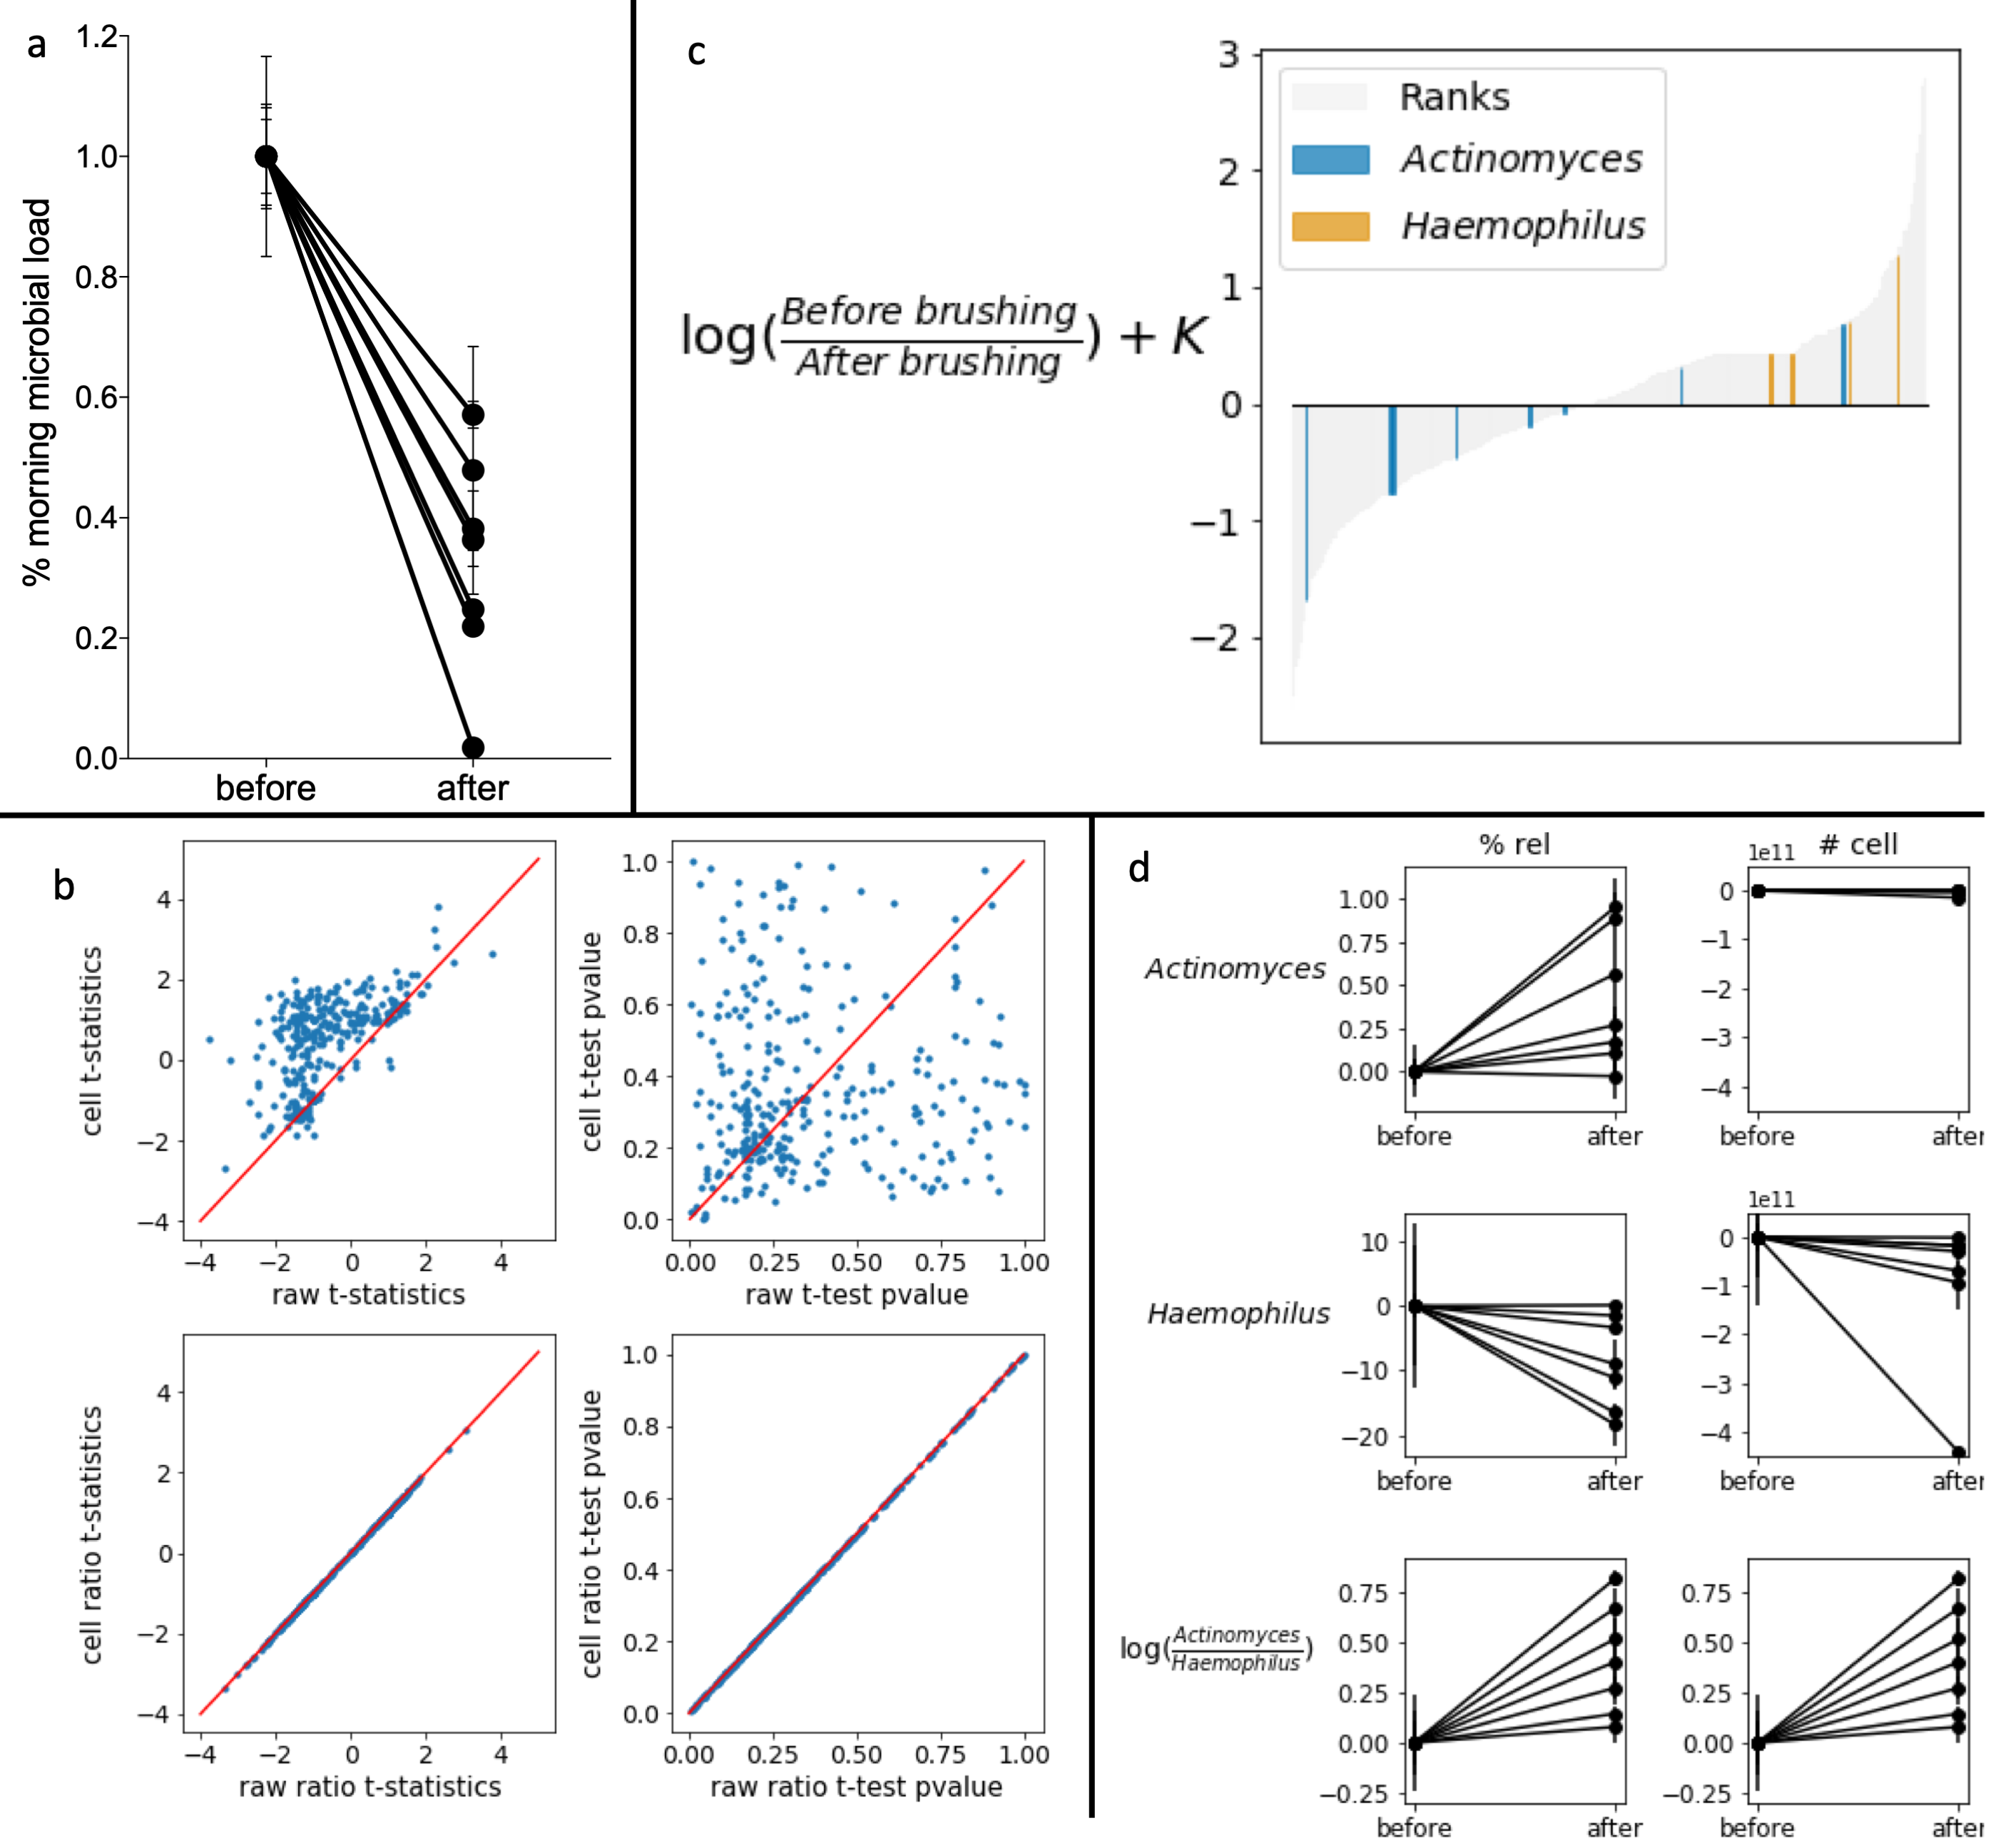
\includegraphics[width=1\textwidth]{ch4/Figure2.png}
  \caption[Comparison of absolute and relative abundance data using proportions, ratios and ranks on
    oral microbial communities.]{
    Analysis of salivary microbiota before and after brushing teeth. (a) Flow cytometry-quantified microbial
    load in unstimulated saliva collected for 5 minutes normalized to before brushing teeth. Each line corresponds
    to a different volunteer. (b) A comparison of t-statistics (left) and p-values (right) on individual taxa (top)
    and ratio between each taxa to \textit{Actinomyces} (bottom) between relative abundance data (x-axis) and cell
    count-normalized data (y-axis). (c) Microbial ranks estimated from multinomial regression applied to oral time
    series dataset with \textit{Actinomyces} and \textit{Haemophilus} highlighted.  The y-axis represents the log-fold change that is
    known up to some bias constant K, and the x-axis numerically orders the ranks of each taxa in the analysis
    (d) A comparison of relative abundance vs cell counts of \textit{Actinomyces}, \textit{Haemophilus} and log(\textit{Actinomyces}:\textit{Haemophilus})
    before and after brushing teeth. Only the differences since the before time point are visualized.}
\end{figure}
%
For both relative abundances and estimated cell counts, we performed paired t-tests to evaluate the change
in abundance of each taxon before and after brushing (Fig. 2b). It is clear that there are numerous false
positives resulting from applying t-tests to relative abundance data, given the disagreements between the
cell normalized and raw t-statistics (Spearman r=$0.53$) and p-values (Spearman r=$0.09$).  On the other
hand, if we instead focus on the ratio between \textit{Actinomyces} and the remaining taxa, the t-statistics and
p-values between the cell normalized and raw data are identical (Spearman r=$1.0$). Consequently, the
ratios are unaffected by microbial load, whereas the raw relative abundance values are affected as to
prevent meaningful inference.
%
From the differentials obtained from the multinomial regression (Fig. 2c), we can identify which taxa are
changing the most (highest and lowest log fold change - Table S1). Here, we highlight \textit{Actinomyces} and
\textit{Haemophilus}, which are on opposite ends of the spectrum. This suggests that \textit{Haemophilus} taxa are more prevalent
before brushing, and \textit{Actinomyces} taxa are more prevalent after brushing. When inspecting t-test results on
individual taxa in the relative abundance data, it appears that \textit{Actinomyces} significantly increased
(t-statistic=$2.89$, p-value=$0.013$) after brushing teeth and that \textit{Haemophilus} significantly decreased
(t-statistic=$-2.593$, p-value=$0.023$). But if we look at the cell counts, only \textit{Haemophilus} significantly
decreased (t-statistic=$-2.477$, p-value=$0.029$) (Fig. 2d). This is expected, because \textit{Haemophilus} is
typically found on the periphery of oral biofilms and was likely washed away during the brushing process,
whereas \textit{Actinomyces} is generally found on the surface of the tooth and acts as an anchor for biofilm
attachment \cite{Welch2016-lw}. \\[5 mm]
%
The log ratio of \textit{Actinomyces} and \textit{Haemophilus} between the relative abundances and the cell counts is identical.
While we cannot observe the decrease of \textit{Haemophilus} or the stability of \textit{Actinomyces}, with the log ratio of their
relative abundance, we can observe the interaction between these two taxa and the increase of \textit{Actinomyces}
relative to \textit{Haemophilus} after brushing teeth (t-statistic=$2.833$, p-value=$0.015$) without having the added
information from absolute abundances. Similarly, the log ratios of each species compared to \textit{Actinomyces} is
consistent between the relative abundance data and the cell normalized data (Fig. 2b, bottom plots).\\[5 mm]
%
This consistency between inferences made based off the relative and absolute abundances is crucial, because
in many circumstances it is not possible or practical to estimate total microbial load. For example, skin swabs
are often difficult to use in flow cytometry due to very low biomass and difficulty in transferring intact cells
from the swab into a liquid solution. Furthermore, skin samples are notoriously sensitive to 16S \gls{rrna} gene primer
choice making \gls{qpcr} quantification challenging. Similarly, for historically collected samples that now exist only
as DNA in a freezer or as sequences in a database, flow cytometry approaches are not feasible. \\[5 mm]
%
\subsection{Discovery of interkingdom relationships in atopic dermatitis}
%\\[5 mm]
The tooth brushing example provides ground truth for the method, but many clinically relevant microbiome questions
involve less obvious differences. We demonstrate how viewing relative abundances alone produces false negatives in
the context of an important skin disease, atopic dermatitis (\gls{ad}). \gls{ad} has a complex etiology, and many microbiome
studies performed using next-generation sequencing have focused on bacterial changes associated with \gls{ad}, with major
focus on the pathogen \textit{Staphylococcus aureus}. The yeast genus \textit{Malassezia} has also been implicated, although conflicting
results have been published as to which \textit{Malassezia} species are involved and whether they are more or less prevalent
in \gls{ad} \cite{Glatz2015-ag}. A recent shotgun metagenomic study examined the skin microbiome over time during an \gls{ad}
flare and recovery. They observed a decrease in \textit{Staphylococcus aureus} relative abundance in the healthy, recovered
skin (non-lesioned) compared to \gls{ad} flare (lesion), but no significant changes in the relative abundance of
\textit{Malassezia} species over time in these \gls{ad} patients \cite{Byrd2017-eb}.
%
However, applying compositionally coherent methods to this dataset revealed part of the story which was missing.
Observing the ranks from multinomial regression (Fig. 3a, TableS2), it is apparent that compared to lesioned skin,
\textit{S. aureus} is one of the taxa to decrease the most relative to all of the microbial species in the non-lesioned sites,
followed by \textit{S. epidermidis}, and \textit{M. globosa}. Consistent with the analysis of proportions
in (Fig. 3b) the ratio of \textit{S. aureus} : \textit{P. acnes} was significantly increased in flare
(t-statistic=$2.973$, p-value=$7.811 \times 10^{-3}$) and correlated with \gls{scorad} score, a clinical assessment
of \gls{ad} severity (Pearson=0.747, p-value=$3.516 \times 10^{-6}$). Contrary to previous findings, both
\textit{S. epidermidis} : \textit{P. acnes} and \textit{M. globosa} : \textit{P. acnes} were also significantly
increased in lesioned skin (t-statistic=$3.197$, p-value=$4.748 \times 10^{-3}$, and t-statistic=$4.030$,
p-value=$7.16 \times 10^{-4}$, respectively) and correlated with SCOR\gls{ad} score (Pearson=0.464,
pvalue=$6.975 \times 10^{-4}$, and Pearson=$0.668$, p-values$1.125 \times 10^{-7}$, respectively) (Fig. 3c). \\[5 mm]
\begin{figure}
  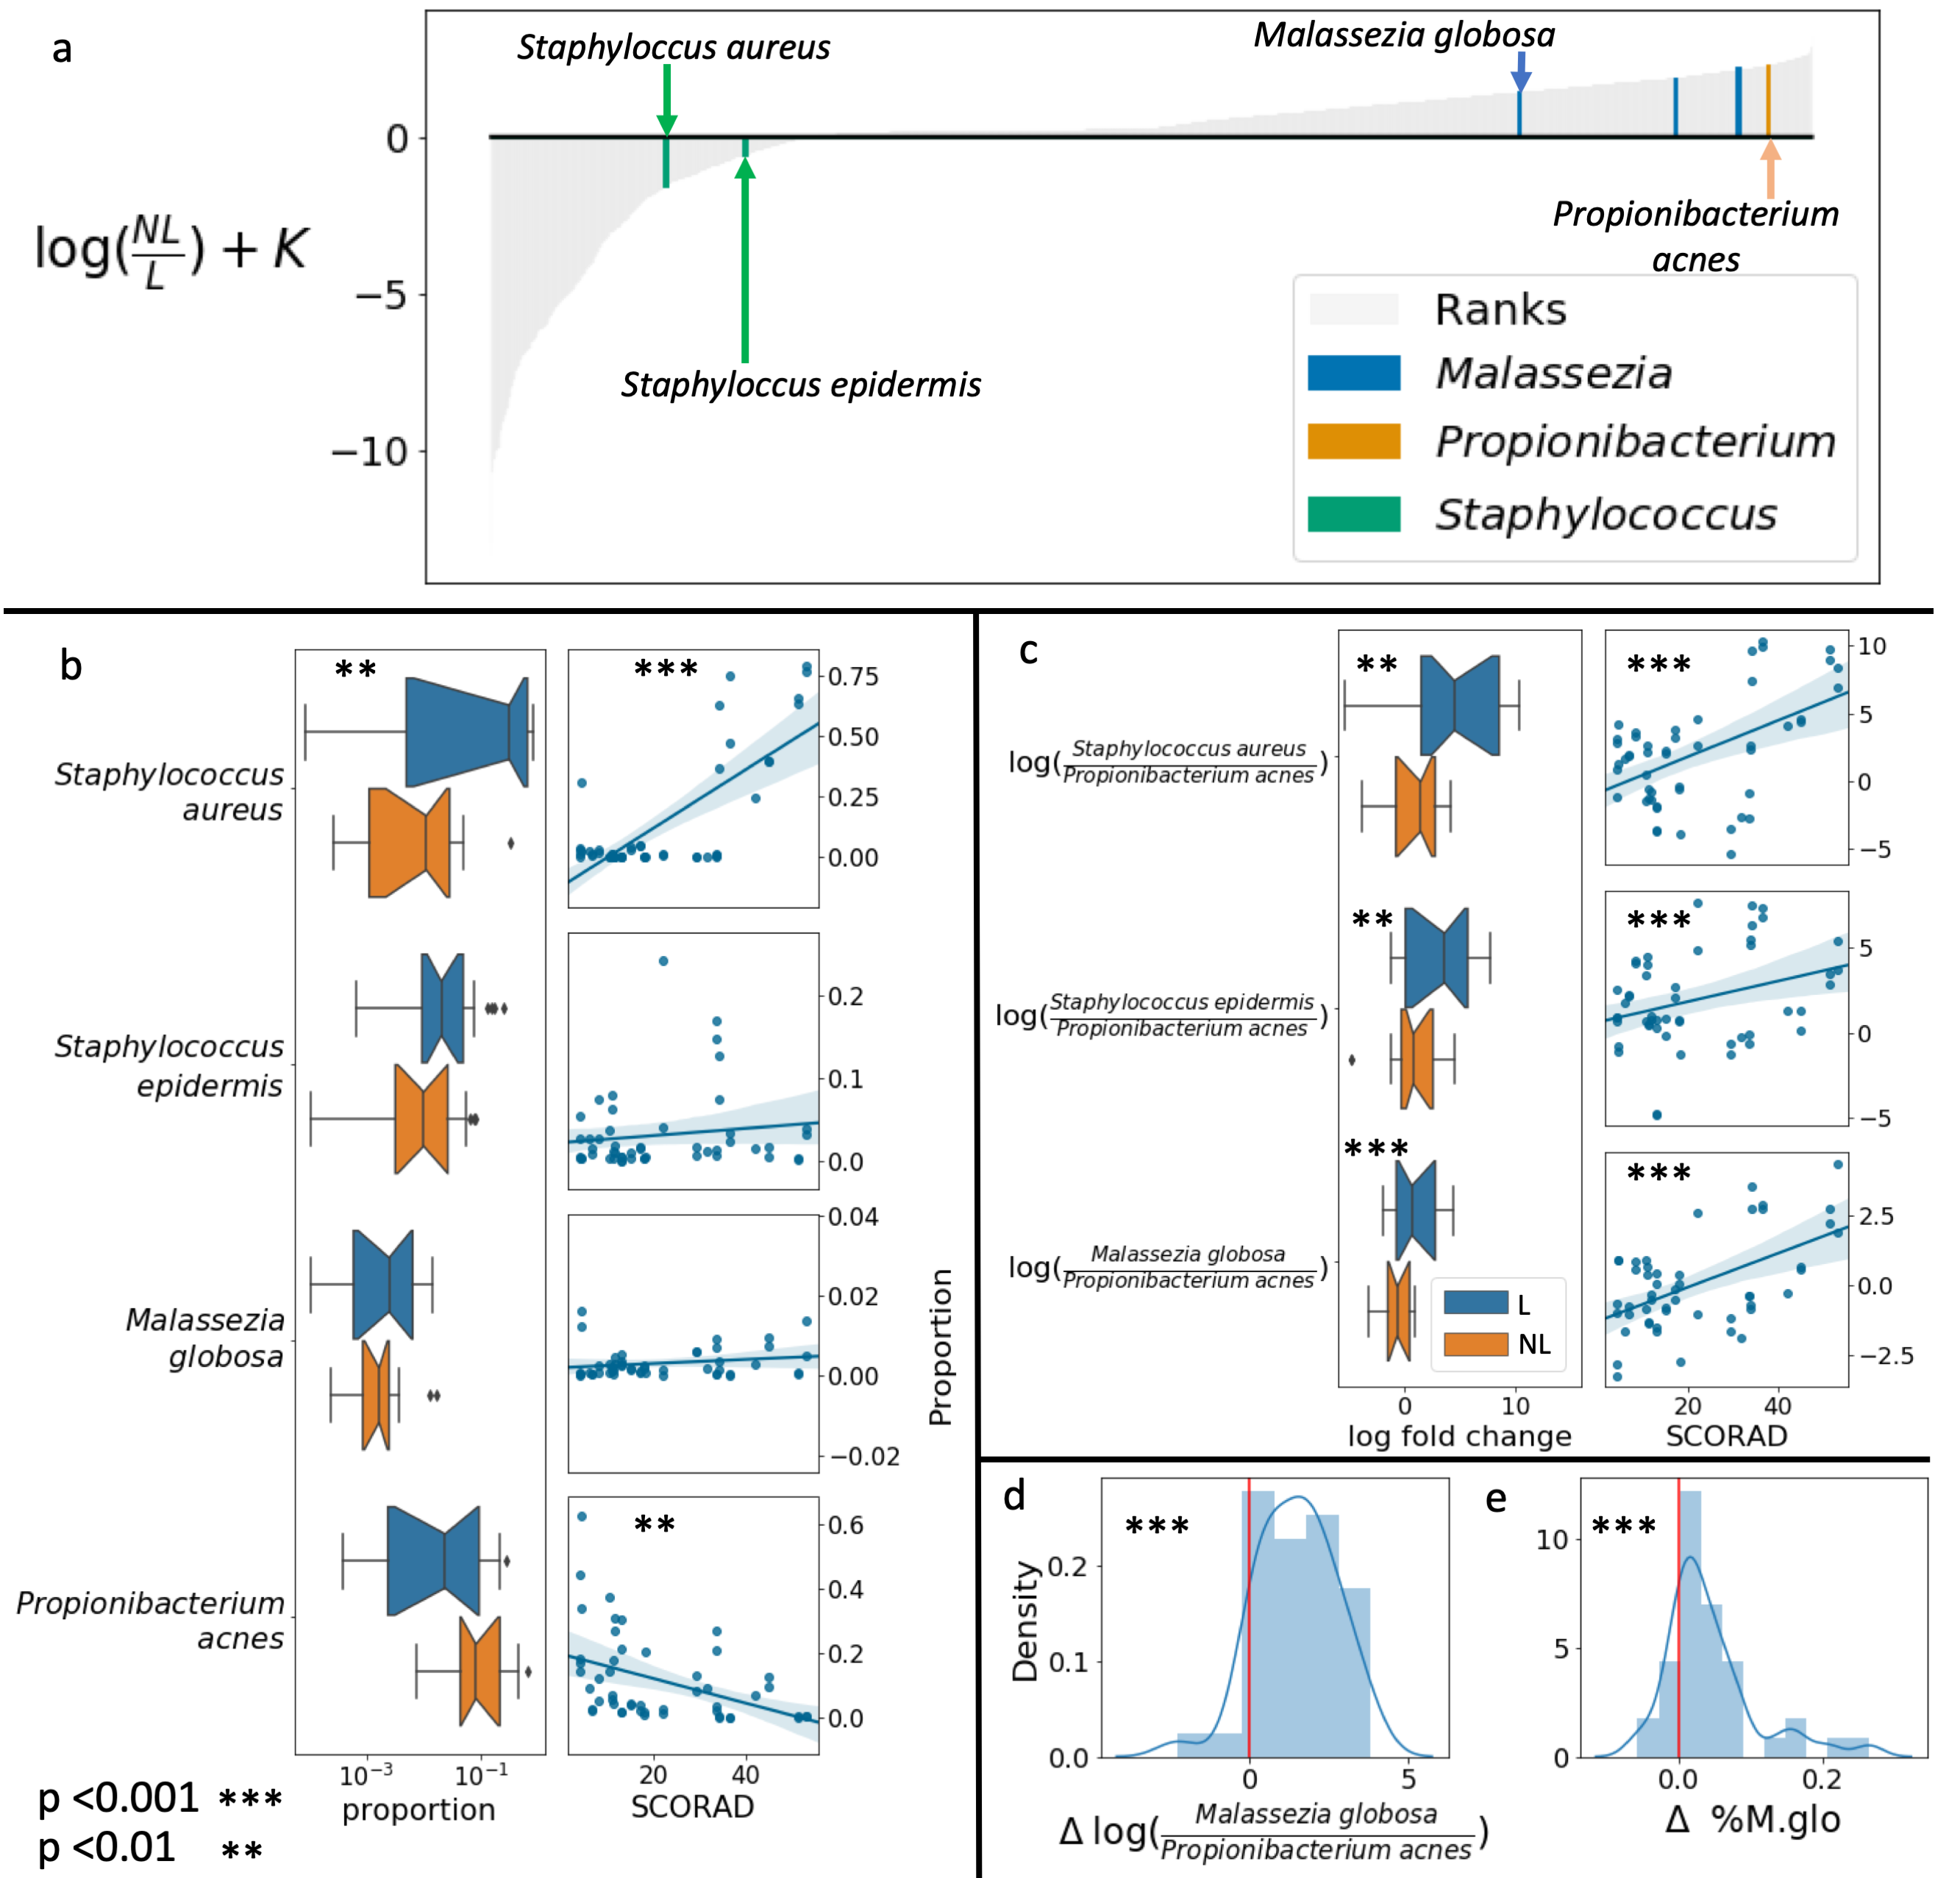
\includegraphics[width=1\textwidth]{ch4/Figure3.png}
  \caption[Analysis of lesion and non-lesion sites using proportions, log-ratios and ranks on two
    independent atopic dermatis cohorts.]{
    Comparison of lesioned (L) versus non-lesioned (NL) skin in two atopic dermatitis studies;
    Byrd et al.\cite{Byrd2017-eb}, (a-c) and Leung et al.\cite{Leung-DYM}, (d-e). (a) Microbial ranks estimated from
    multinomial regression applied to shotgun metagenomics from Byrd et al\cite{Byrd2017-eb} with key
    genera highlighted. The y-axis represents the log-fold change that is known up to some bias constant K.
    (b) Proportions of \textit{S. aureus}, \textit{S. epidermidis}, \textit{M. globosa}, and \textit{P. acnes}
    in lesioned (blue) and non-lesioned (orange) skin (left) and correlation of relative abundance
    with \gls{scorad} score (right) (c) Log-ratios of \textit{S. aureus} : \textit{P. acnes} , \textit{S. epidermidis} : \textit{P. acnes} ,
    and \textit{M. globosa} : \textit{P. acnes} (left) and correlation of ratio with \gls{scorad} score.
    (d) Change in log ratio of \textit{M. globosa} : \textit{P. acnes}. (e) Change in
    relative abundance of M. globosa between lesioned and non-lesioned skin from (Leung et al.\cite{Leung-DYM}).}
\end{figure}
%
To validate this observation, we analyzed shotgun data from another atopic dermatitis dataset (Leung et al. \cite{Leung-DYM}, under review).
Again, we found that although there was no difference in the proportion of M. globosa between lesioned and non-lesioned skin
(Fig. 3e), the ratio of \textit{M.globosa} : \textit{P.acnes} increased significantly in lesioned skin (t-statistic=$5.79$,
p-value=$8.6 \times 10^{-7}$) (Fig. 3d). These results are congruent with a previous finding that \textit{M. globosa}
was cultivated more successfully from lesioned versus non-lesioned sites in \gls{ad} \cite{Falk2005-we}. Analysis
differentials can identify a novel, clinically significant microbial interaction which can be validated
across cohorts by choosing insightful reference frames for measuring compositional change.\\[5 mm]
%
\section*{Discussion}
Adding information about absolute microbial load between samples can highlight issues inherent in compositional data
analysis. However, there are multiple practical and technical challenges in applying flow cytometry, \gls{qpcr}, or culturing
analyses to complex or low biomass sample types such as skin swabs. Fortunately, absolute abundances of a community
are only one dimension of measurement and there are robust, alternative techniques forgoing the need to estimate total
biomass. We have demonstrated the validity of using microbial ratios and ranked differentials to determine significant
changes in microbiome studies by comparing compositional inferences with absolute abundance inferences. \\[5 mm]
%
By using flow cytometry to quantify total microbial load, we were able to validate these analytical tools in 16S \gls{rrna} gene
amplicon sequencing data from unstimulated saliva. We found evidence of false positives when looking exclusively at changes
in relative abundance before and after brushing teeth. By looking at the ratio of \textit{Actinomyces} : \textit{Haemophilus}, we reached
an identical conclusion to our cell-count normalized data without the need for microbial load quantification. The
consistency of our results rests from the use of ratios defining reference frames for inferring compositional changes.
Other methods for inferring community compositional changes with different reference frames can be assumed to be
similarly reliable and bypass the need for costly and rate-limiting absolute abundance data.
%
Furthermore, we highlighted an example of a false negative in previously generated shotgun metagenomic data from the
skin of individuals with \gls{ad}. We were able to reproduce the findings that \textit{S. aureus}, and to a lesser extent S. epidermidis,
are differentially abundant in \gls{ad} lesions. Additionally, using log ratios and differential ranking, we were also able
to show a more subtle but statistically significant change in \textit{M. globosa} abundance in \gls{ad} lesions. This same result was
obtained in two independent metagenomic studies of \gls{ad} patients, and agrees with previous culturing-based work quantifying
increased colony forming units of \textit{M. globosa} in \gls{ad} lesions. \\[5 mm]
%
The seeming contradiction between microbial load-corrected abundances and relative abundances does not invalidate data
from the existing 40,000+ experiments utilizing 16S \gls{rrna} gene amplicon or metagenomic sequencing. Importantly, these
techniques are not limited to next generation microbiome sequencing, but can be applied to any experiments involving
compositional data (e.g. metabolomics, transcriptomics, proteomics, etc.). \\[5 mm]

While there are widespread misconceptions concerning how to interpret microbial abundances, there is still much
hope for resolving these outstanding controversies. Ongoing efforts at the NIH and EMBL-EBI have already stored
multiple petabytes of multi-omics datasets ready to re-analyze, databases such as Qiita contain curated data and
metadata from hundreds of thousands of samples \cite{Gonzalez2018-rv} , and there is much promise for resolving
the outstanding controversies by analyzing these datasets using reference frames to make stable inferences of
compositional change. \\[5 mm]
%
%
\section{Methods}
If we wanted to compute the change between two samples containing compositions (e.g. relative abundance of microbes) $\bm A=(a_1,...,a_D)$ and $\bm B=(b_1,...,b_D)$ , it would look like
\begin{align}
  \frac{\bm{A}}{\bm{B}}=\big(\frac{a_1}{b_1} ,\ldots  \frac{a_D}{b_D}\big)
\end{align}
If we are only able to measure relative abundances, as is the case with next generation amplicon sequencing, we can only estimate the proportion $p_{a_i}$ for species $i$ in the sample $A$  i.e. $p_{a_i}=\frac{a_i}{N_a}$.  Estimating the true abundance can be done via $a_1=N_a p_{a_1}$, where $N_a$ is the total abundance of sample $A$.  If we wanted to estimate the true change, that can be done as follows
\begin{align}
  \frac{\bm{A}}{\bm{B}} =
  \frac{N_a \times p_{a_1}}{N_b \times p_{b_1}}, \ldots \frac{N_a \times p_{a_D}}{N_b \times p_{b_D}} =
  \frac{\bm{p_A}}{\bm{p_B}} \times  \frac{\bm{N_A}}{\bm{N_B}}
\end{align}
If we wanted to determine if species $i$ abundance has changed between samples $A$ and $B$, we would want to test to see if $\frac{a_i}{b_i}=1$. However as shown above, we cannot perform this test, since the results of this test would be confounded by the total biomass bias $\frac{N_A}{N_B}$.\\[5 mm]
In many cases, the total biomass cannot be estimated, so any techniques to identify important species will need to alleviate this bias. One alternative is to use ratios. If we choose species D to be the reference species, it is clear that the total biomass cancels as follows
\begin{align}
  \frac{a_1/a_D}{b_1/b_D}  =  \frac{p_{a_1}/p_{a_D} }{p_{b_1}/p_{b_D}}
\end{align}
Another alternative is to use ranks. Since the bias is applied uniformly across the differential, it will not affect the ordering of the species. Hence, ranks are agnostic to the total biomass bias.
\begin{align}
  rank (\frac{\bm{A}}{\bm{B}}) =
  rank(\frac{\bm{p_A}}{\bm{p_B}} \times \frac{\bm{N_A}}{\bm{N_B}}) =
  rank(\frac{\bm{p_A}}{\bm{p_B}} )
\end{align}
This differential is also commonly referred to as a perturbation in the context of the compositional literature \cite{Pawlowsky-Glahn2015-qb}.
It is important to note that this does not justify using Spearman correlation or other non-parameteric tests such as Kruskal-Wallis applied to relative abundance data since these tests do not satisfy scale invariance \cite{Friedman2012-cn}.\\[5 mm]
%
Both of these techniques satisfy scale invariance, meaning that both of these techniques are agnostic to the total biomass.  This concept is critical when analyzing relative abundance data, since this is one step closer to maintaining consistent conclusions between the original environment and the observed sequences.\\[5 mm]
%
Estimating log-fold differential expression from relative abundances can result in either false positive (\gls{fp}) or false negatives (\gls{fn}) depending on the distribution of true differential expression. Whether \gls{fn}s or \gls{fp}s are observed depends on a nonlinear relationship involving the true (unobserved) differential expression. For a p-vector $x$ let us define $\gls{lse}(x) = \log(e^{x_1}+ \ldots +e^{x_p})$. If $\bm{\delta}=(\delta_1, \ldots ,\delta_D)$ denotes the true differential expression of the $D$ species between two conditions, let $\bm{\alpha}=\gls{lse}(\bm{\delta})$. Further, let $\hat{\bm{\delta}}=(\hat{\delta_1}, \ldots, \hat{\delta_D})$ represent the inferred differential expression from proportional data and $\bm{\hat{\alpha}}=\gls{lse}(\bm{\hat{\delta}})$. If $\gls{lse}(\delta) > \gls{lse}(\hat{\delta})$ then \gls{fp}s will be observed. In contrast if $\gls{lse}(\delta) < \gls{lse}(\hat{\delta})$ then \gls{fn}s will be observed.\\[5 mm]
%
\subsection{Saliva sample collection}
Eight volunteers provided unstimulated saliva so that salivary flow rate could be measured according to a standardized protocol \cite{Navazesh2008-me}. Briefly, individuals were asked to allow saliva to flow for exactly five minutes through a disposable funnel (Simport, SIM F490-2)into a sterile, 15 mL conical tube preloaded with 2 mL sterile glycerol for bacterial preservation. Participants were asked to provide samples before brushing and after brushing teeth in the morning and in the evening. Samples inverted several times to mix with the glycerol and stored at -20$\degree$C immediately after collection. This study was approved by an Institutional Review Board (IRB\# 150275) and written informed consent was acquired before sample collection\\[5 mm]
%
\subsection{Flow cytometry}
Unstimulated saliva samples were thawed on ice, and aliquots were diluted tenfold with sterile, 1x PBS. To remove human cells and salivary debris, samples were filtered using a sterile 5 $\mu$m syringe filter (Sartorius Stedim Biotech GmbH). 5 $\mu$l 20x SYBR green (SYBR$^{TM}$ Green I Nucleic Acid Gel Stain, Invitrogen) was added to 1 mL of the microbial suspension (0.1x final concentration) and incubated in the dark for 15 minutes at 37$\degree$C.  Finally, 50 $\mu$l AccuCount Fluorescent Particles (Spherotech, AC\gls{fp}-70-10) were added for assessment of microbial load. Sample were processed on a SH800 Cell Sorter (Sony Biotechnology) using a 100 $\mu$m chip with the threshold set on FL1 at 0.06\%, and gain settings as follows; FSC=4, BSC=25\%, FL1=43\%, FL4=50\%. The gating strategy was adapted from Vandeputte et al.,\cite{Vandeputte2017-jl}. Briefly, fluorescent microbial cells were gated from background on a FL1-Fl4 density plot, and remaining background was removed by eliminating large events detected on a FSC-BSC density plot. Negative controls (sterile PBS stained identically to samples) was run between each sample set to exclude cross-contamination. Settings were identical among all samples.\\[5 mm]
%
\subsection{Amplicon sequencing}
DNA extraction and 16S \gls{rrna} amplicon sequencing were done using Earth Microbiome Project (EMP) standard protocols (http://www.earthmicrobiome.org/protocols-and-standards/16s). 500 $\mu$l of unstimulated saliva was used for gDNA extraction with MagAttract PowerSoil DNA Kit (QIAGEN) as previously described \cite{Marotz2017-dy}. Amplicon PCR was performed on the V4 region of the 16S \gls{rrna} gene using the primer pair 515f to 806r with Golay error-correcting barcodes on the reverse primer. 240 ng of each amplicon was pooled and purified with the MO BIO UltraClean PCR cleanup kit and sequenced on the Illumina MiSeq sequencing platform.\\[5 mm]
The sequences and biom tables \cite{McDonald2012-xw} can be found on Qiita (http://qiita.microbio.me) under study ID 11896. Demultiplexed fastq files were processed using QIIME2 (https://qiime2.org)\cite{Caporaso2010-nm}.  Deblur was used to denoise the sequences \cite{Amir2017-zw}.  16S taxonomy was assigned using RDP classifier \cite{Pawlowsky-Glahn2015-qb,Wang2007-gj}. Songbird was used to perform multinomial regression - repository can be found here: https://github.com/mortonjt/songbird\\[5 mm]
Paired t-tests were performed to evaluate the differences before and after brushing teeth.
All log-ratios that were evaluated to either positive or negative infinity are dropped prior to statistical analysis.
These numerical issues occur due to particular microbes not observed, and we treat them as missing data respectfully.
%
\subsection{Shotgun metagenome studies}
We used supplementary data from Byrd et al \cite{Byrd2017-eb} and Donald Leung\cite{Leung-DYM}. The provided relative abundances were compared to the log ratio of the raw count data. Paired t-tests were performed to evaluate the differences between lesion and non-lesion skin samples.
All log-ratios that were evaluated to either positive or negative infinity are dropped prior to statistical analysis.
These numerical issues occur due to particular microbes not observed, and we treat them as missing data respectfully.

\section{Acknowledgements}
We would like to Doris Vandeputte for her insights behind the total microbial load quantification.
J.T.M. was funded by NSF GR\gls{fp} DGE-1144086.
